\documentclass{article}
\usepackage[utf8]{inputenc}

\usepackage[margin=1in]{geometry} % Useful for setting margins
% \usepackage[showframe]{geometry} % Uncomment to see the margin bounding boxes. Useful for proofing
% Use \newgeometry{} and \restoregeometry to alter margins on the fly
% Documentation: https://www.ctan.org/pkg/geometry
\usepackage{siunitx} % Useful for typesetting units and scientific notation
% Use with \SI{}; \num{}; \ang{}
% Documentation: https://www.ctan.org/pkg/siunitx
\usepackage{chemformula} % Useful for typesetting chemical formulae 
% Use with \ch{}
% Documentation: https://www.ctan.org/pkg/chemformula
\usepackage{miller} % Useful for typesetting miller indices
% Use with \hkl<>; \hkl[]; \hkl(); \hkl{}
% Documentation: https://www.ctan.org/pkg/miller
\usepackage[labelfont=bf]{caption} % For captioning figures
\usepackage{subcaption} % For captioning subfigures
\usepackage{lineno} % For adding line numbers
\usepackage{hyperref} % Automatically adds clickable hyperlinks between sections and refs
\usepackage{graphicx} % Allows embedding images
\usepackage{float} % More precise figure placement
\usepackage{newfloat} % Allows creation of new floating environments. Only import if necessary
\usepackage{amsmath,amssymb} % Math environments and symbols
\usepackage{listings} % Allows syntax-highlighted inline code
\usepackage{tikz} % Commonly used package for 2D drawing
\usepackage[inline]{asymptote} % Used for drawing 3D diagrams
\usepackage{cancel} % Adds a quick macro for striking through math terms
\usepackage{chemfig} % Adds a programmatic way to draw chemical structure images
\usepackage{xcolor} % Adds the ability to change text color. May interact poorly with printers
\usepackage{url} % Makes typesetting urls easier
\usepackage{lmodern} % Different font with more features

%%%%%%%%%%%%%%%%%%%%%%%%%%%%%%%%%%%%%%%
% Honorable Mentions
%%%%%%%%%%%%%%%%%%%%%%%%%%%%%%%%%%%%%%%
% These packages solve very specific problems and I don't typically import them
%%%%%%%%%%%%%%%%%%%%%%%%%%%%%%%%%%%%%%%
% \usepackage{wrapfig}
% Allows wrapped figures and tables. Use at your own risk

% \usepackage[explicit,compact,small]{titlesec}
% Manipulates titles and sections, to make them more compact. 
% Useful on NSF proposals

% \usepackage{beamer}
% For making presentations using LaTeX

% \usepackage{microtype}
% Makes small tweaks to typesetting to make things more compact.
% Useful on NSF Proposals

%%%%%%%%%%%%%%%%%%%%%%%%%%%%%%%
% Declare Custom SI units
%%%%%%%%%%%%%%%%%%%%%%%%%%%%%%%
\DeclareSIUnit[quantity-product = \,]
\rpm{\text{rpm}}


\begin{document}
\definecolor{codegreen}{rgb}{0,0.6,0}
\definecolor{codegray}{rgb}{0.5,0.5,0.5}
\definecolor{codepurple}{rgb}{0.58,0,0.82}
\definecolor{backcolour}{rgb}{0.95,0.95,0.92}

%Code listing style named "mystyle"
\lstdefinestyle{mystyle}{
  backgroundcolor=\color{backcolour}, commentstyle=\color{codegreen},
  keywordstyle=\color{magenta},
  numberstyle=\tiny\color{codegray},
  stringstyle=\color{codepurple},
  basicstyle=\ttfamily\footnotesize,
  breakatwhitespace=false,         
  breaklines=true,                 
  captionpos=b,                    
  keepspaces=true,                 
  numbers=left,                    
  numbersep=5pt,                  
  showspaces=false,                
  showstringspaces=false,
  showtabs=false,                  
  tabsize=2
}

%"mystyle" code listing set
\lstset{style=mystyle}
\begin{center}
    \LARGE \textsc{Useful Packages}
\end{center}
%
\section{Scientific Typesetting}
%
    \subsection{SIUNITX}
%
\verb|siunitx| provides many useful commands for typesetting units and numbers both inside and outside math environments. 
For example:
\begin{itemize}
    \item Input: \verb|\SI{2E-5}{\eV\per\nm\squared}|
    \item Output: \SI{2E-5}{\eV\per\nm\squared}
    \item Input: \verb|\num{10.0E-3}|
    \item Output: \num{10.0E-3}
    \item Input: \verb|\ang{30}|
    \item Output: \ang{30}
    \item Input: \verb|\SI{200}{\degreeCelsius}|
    \item Output: \SI{200}{\degreeCelsius}
\end{itemize}
If a unit is not SI, but you would like to use it with the package you can define custom units by declaring them in the document preamble, as mentioned in the package documentation:\\
\verb|\DeclareSIUnit[quantity-product = \,]|\\
\verb|\rpm{\text{rpm}}|\\
This can now be used like any other SI unit:
\begin{itemize}
    \item Input: \verb|\SI{2000}{\rpm}|
    \item Output: \SI{2000}{\rpm}
\end{itemize}
%
    \subsection{Chemformula}
%
\verb|chemformula| provides simple macros for typesetting chemical formulae:
\begin{itemize}
    \item Input: \verb|\ch{H2SO4}|
    \item Output: \ch{H2SO4}
\end{itemize}
%
    \subsection{Miller}
%
\verb|miller| provides excellent macros for typesetting crystal indices:
\begin{itemize}
    \item Input: \verb|\hkl<10-12>|
    \item Output: \hkl<10-12>
\end{itemize}
All standard closures are supported ($<>$, \{\}, [], ())
%
    \subsection{Listings}
%
\verb|listings| provides support for blocks of syntax-highlighted code within LaTeX documents:
\begin{lstlisting}[language=Python]
a = 1
b = 'two'
for i in range:
    print(i)
\end{lstlisting}
The syntax highlighting is defined in the \verb|codestyling.tex| file, and can be modified as desired.
The \verb|codestyling.tex| file must be \verb|input| into the document before it can be used.
%
\section{Graphics and Drawing}
%
    \subsection{Chemfig}
%
\verb|chemfig| provides rich support for creating nicely programmatically drawn chemical structures in LaTeX documents.
The necessary syntax is somewhat confusing, but looking at the documentation is quite helpful.
\begin{itemize}
    \item Input: \verb|\chemfig{*6(-=-=(-([::60]=O)-[::-60]OH)-=)}|
    \item Output: \chemfig{*6(-=-=(-([::60]=O)-[::-60]OH)-=)}
\end{itemize}
%
    \subsection{TikZ}
%
\verb|tikz| is the most commonly used 2D graphics package in the LaTeX world, and can do most things that you would want.
It's quite useful for drawing diagrams, and small figures, but it can even be used to plot data from a \verb|csv| file with the correct setup.\\
\begin{tikzpicture}
\draw[gray, thick] (-4,0) -- (-2,0);
\draw[gray, thick] (-3,1) -- (-3,0);
\draw[gray, thick] (4,-1) -- (2,-1);
\draw[gray, thick] (3,-1) -- (3,-2);
\draw[gray, ultra thick, ->] (-2.5,0.5) -- (0,0.5);
\draw[gray, ultra thick, ->] (2.5,-1.5) -- (0,-1.5);
\end{tikzpicture}
%
    \subsection{Asymptote}
%
\verb|asymptote| provides both 2D and 3D graphics primitives.
It has its own graphics language, so it can be somewhat challenging to get what you want out of it.
The build system can also have difficulties with updating things on overleaf, but when you get it working, it's quite capable.\\
\begin{asy}
    size(5cm,0);
    import three;
    import palette;
    currentprojection=orthographic(3,1,1);
    draw((1,0,0)--(1,1,0)--(0,1,0)--(0,1,1)--(1,1,1)--(1,0,1)--(0,0,1)--(0,1,1));
    draw((1,1,0)--(1,1,1));
    draw((1,0,0)--(1,0,1));
    draw((0,0,0)--(1,0,0),dashed);
    draw((0,0,0)--(0,0,1),dashed);
    draw((0,0,0)--(0,1,0),dashed);
    draw((0,0,0)--(0,0,-1),dashed);
    draw((0,1,0)--(0,1,-1),dashed);
    draw(surface((1,0,0)--(0,0,-1)--(0,1,-1)--(1,1,0)--cycle),blue+opacity(0.2),nolight);
    draw((1,0,0)--(1.5,0,0),Arrow3);
    label("$+x$",(1.5,0,0),S);
    draw((0,1,0)--(0,1.5,0),Arrow3);
    label("$+y$",(0,1.5,0),S);
    draw((0,0,1)--(0,0,1.5),Arrow3);
    label("$+z$",(0,0,1.5),N);
    label("$(10\bar{1})$",(1,0.5,-0.5),NE);
\end{asy}
%
    \subsection{Subcaption}
%
\verb|subcaption| allows for the creation of subfigures within a document.
It's quite useful for prototyping figures and moving them around prior to committing to a final arrangement.
Labels can be placed on subcaptions which can then be referenced in the text.
\begin{figure}[H]
    \centering
    \begin{subfigure}{0.6\textwidth}
        \centering
        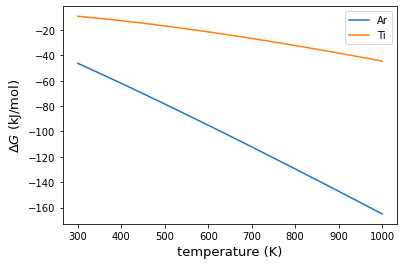
\includegraphics[width=\textwidth,keepaspectratio]{figures/DeltaG.png}
        \caption{}
        \label{fig:example1}
    \end{subfigure}
    \begin{subfigure}{0.3\textwidth}
        \begin{subfigure}{\textwidth}
            \centering
            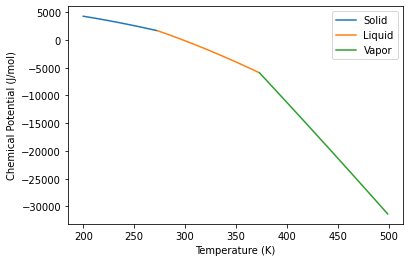
\includegraphics[width=\textwidth,keepaspectratio]{figures/equilibriumplot.png}
            \caption{}
            \label{fig:example2}
        \end{subfigure}
        \begin{subfigure}{\textwidth}
            \centering
            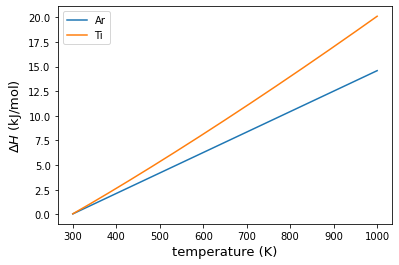
\includegraphics[width=\textwidth,keepaspectratio]{figures/DeltaH.png}
            \caption{}
            \label{fig:example3}
        \end{subfigure}
    \end{subfigure}
    \caption{
    (\subref{fig:example1}) basic demonstration of the subref command for a subfigure.
    (\subref{fig:example2}) The other subfigure.
    (\subref{fig:example3}) the last subfigure.
    }
    \label{fig:example-main}
\end{figure}
This is a somewhat more complicated example, but it shows that you can nest subfigures to obtain quite complicated layouts.
The resulting figures can be referenced as usual, e.g. Figure \ref{fig:example2}.
Using the ref command will give a full reference, and using the subref command will give only the subreference, e.g. Figure \ref{fig:example-main} part (\subref{fig:example2}).
%
    \subsection{PGFplots and CSVsimple}
%
The combination of \verb|pgfplots| and \verb|csvsimple| allows for the reading of data, and plotting all within the LaTeX environment.
For example:
\begin{figure}[H]
    \centering
    \begin{tikzpicture}
        \begin{axis}[
        axis line style = thick, % Self-explanatory
        every x tick/.style={color=black,thick},
        every y tick/.style={color=black,thick},
        no markers, % Get rid of the default scatter plot
        xmin=400, % Set x bounds
        xmax=700, % ""
        xlabel={\textbf{Wavelength ($\lambda$) (nm)}}, % Provide X axis label
        ylabel={\textbf{Absorbance (a.u.)}}, % Provide Y axis label
        minor y tick num = {1}, % Number of ticks between major ticks
        yticklabel style={/pgf/number format/fixed}, % Tell PGF Plots not to use exponential notation for y axis ticks
        extra y ticks = {0}, % Add an extra y tick
        extra y tick style = {grid=major}, % Add a horizontal line
        every axis plot/.append style={ultra thick}, % Thicken the plotted lines 
        tick label style={font=\normalsize},
        label style={font=\normalsize}
        ]
            \addplot table [x = Wavelength (nm), y = Absorbance (AU), col sep=comma] {data/30ULALI.csv}; % Import the data. The x and y column labels have to be exactly the same as what they are in the raw data file
            \addplot table [x = Wavelength (nm), y = Absorbance (AU), col sep=comma] {data/30UL.csv};
        \end{axis}
    \end{tikzpicture}
    \caption{This is a test figure to demonstrate plotting a UV-Vis spectrum from raw data inside the LaTeX environment}
    \label{fig:testfig}
\end{figure}
\noindent Much of the boilerplate can be eliminated by defining a custom style:
\begin{figure}[H]
    \centering
    \begin{tikzpicture}
        \begin{axis}[
            UVVis,
            xmin=400,
            xmax=700,
            ]
            \addplot table [x = Wavelength (nm), y = Absorbance (AU), col sep=comma] {data/30ULALI.csv};
            \addplot table [x = Wavelength (nm), y = Absorbance (AU), col sep=comma] {data/30UL.csv};
        \end{axis}
    \end{tikzpicture}
    \caption{This is another test figure showing the use of a predefined style template to cut down on boilerplate code.}
    \label{fig:template}
\end{figure}
In principle, this approach can also be used to auto-populate tables, but I haven't been able to get it to work within Overleaf.

\end{document}
